\section{Real-world challenges to physical-layer identification}
\label{sec:results2}
Using our high-precision fingerprint technqiue, we perform an empirical analysis in lab conditions to understand the limitations of this physical layer identification.
%
There are five primary challenges that limit the effectiveness of tracking
BLE devices based on their physical-layer fingerprint. 
%
For each challenge, we
perform controlled experiments or theoretical analysis to investigate how significantly they affect
fingerprinting accuracy in practice, and in turn the ability of an attacker to uniqely identify their target. 
%
We found that BLE tracking attacks are
likely to be feasible in practice. 
%
However, the attacker's ability to identify a
specific device reliably will vary depending on several factors that are out of
their control.

\subsection{Uniqueness of BLE fingerprints} %{{{
\label{sec:similarity}

\begin{figure}
    \centering
    \captionsetup{justification=centering}
    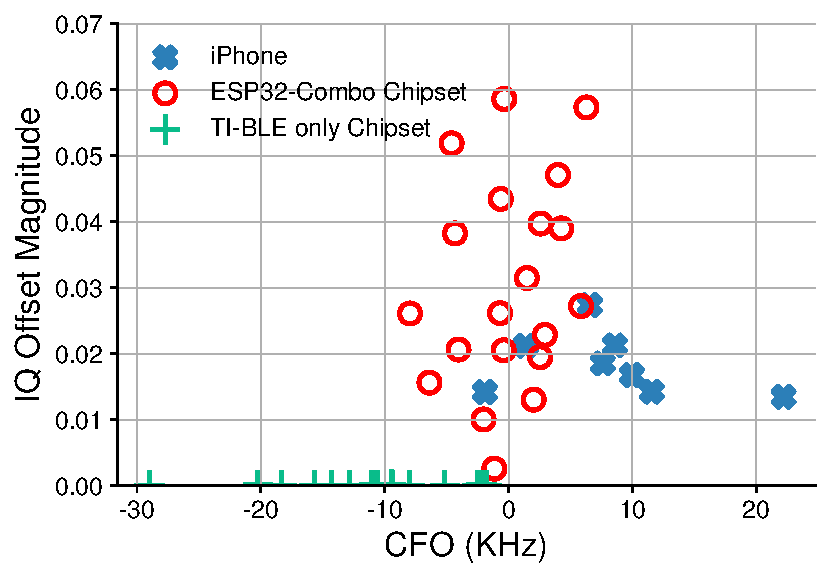
\includegraphics[width = 0.6\linewidth]{bletracking/plots/cfoiq_iphone_esp_ti2.pdf} 
    \caption{Comparing the fingerprints of 48 BLE chipsets}
\label{fig:cfoiq}
\end{figure}

BLE transmitters must have unique imperfections if an attacker wants to
differentiate their target from other nearby devices.  To evaluate how
similar BLE fingerprints are in practice, we compare the fingerprint of  many
devices across three different popular BLE chipsets. Specifically, we
captured the fingerprint of eight recent iPhones with WiFi+BLE combo
chipsets, 20 ESP32 WiFi+BLE microcontroller chipsets, and 20 TI CC2640
BLE-only chipsets used in low-power devices (e.g., fitness trackers).  We
captured 100 packets using a high-quality SDR (USRP N210) from each of these
devices in a controlled environment (i.e., an RF isolation chamber). We
computed the fingerprint of each device across all 100 packets using the methodology described in
the previous section.

Figure~\ref{fig:cfoiq} shows the mean of the fingerprint metrics for each of
the 48 devices. We plot only the CFO and \iq offset metrics to simplify the
visualization, adding \iq imbalance does not change the conclusions of the
experiment. Overall, most of the 48 devices have unique fingerprints. However, there
are a few devices that have similar fingerprints, making them more difficult to uniquely identify. The distribution of
device fingerprints also appears to be dependent on the chipset.
%All devices appear to have
Namely, there are striking differences in how the \iq offset metric is
distributed between different chipsets.
For instance, the ESP32 devices have a much
larger range of \iq offsets than the iPhones, which may be
because ESP32s are low-end chipsets compared to the
high-performance WiFi+BLE combo chipsets used in iPhones.

\begin{figure}
    \centering
    \captionsetup{justification=centering}
    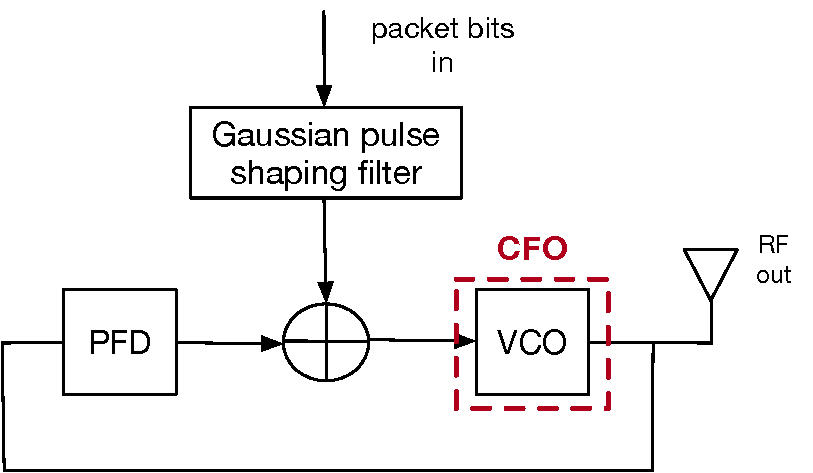
\includegraphics[width = 0.6\linewidth]{bletracking/plots/dpll.pdf} 
    \caption{TI's BLE-only transmitter. This is not an \iq modulator.}
    \label{fig:dpll}
\end{figure}

Surprisingly, the TI BLE-only chipsets all have negligible \iq offset.
Recall in Section~\ref{sec:methodology}, we described how unlike WiFi, BLE is
not an inherently \iq modulated protocol; therefore, the TI's BLE-only
chipset may have \iq offset because it may not use an \iq modulator.  We
confirmed this suspicion by finding a technical report that describes the
TI BLE chipset radio architecture: it uses a PLL-based 
(non-\iq) modulator~\cite{pllarchBLE}.

\subsubsection*{Summary} An attacker's ability to uniquely identify a target device's 
fingerprint depends on the BLE chipset it is using, as well as the
chipsets of the other devices nearby. Distinguishing devices
with the same chipset is likely more difficult than distinguishing 
devices with different chipsets. This may make tracking 
attacks difficult in practice because targets are likely to use the same popular devices (e.g.,
iPhone). %Although, if the target happens to be a device that is not common in that
%environment, they are likely to have a much more unique fingerprint.

%ability to identify a device totally depends on its inherent RF fingerprints.
%There are regions that include many devices with common fingerprints while some
%devices have a very unique and distinguishable fingerprints. Second, although
%most devices seem separable, the fingerprints of some of them are not that far
%from each other. Consequently, a coarse grained imperfection estimation
%algorithm may result in poor accuracy, which emphasizes employing a
%fine-grained imperfection estimation algorithm similar to the one introduced in
%this paper. Also any environmental effect such as noise which increases the
%imperfection estimation error or temperature variations which changes the
%fingerprints, can cause confusion in distinguishing the devices with close
%signatures.

%enough fingerprints to distinguish them. Also, these distributions of
%imperfections may be chipset model specific, some may be easier to distinguish
%than others.
%}}}

\subsection{Temperature stability of BLE fingerprints} %{{{
\label{sec:challenges:temperature} A device's BLE fingerprint must be stable
to track over time across multiple locations.  However, a device's CFO
may drift when the temperature of the device changes.  CFO is a
product of imperfections in the crystal oscillator used to generate the
transmitter's center frequency (e.g., 2.480~GHz), and the frequency error of
a crystal oscillator has a well-defined relationship with its temperature
called the ``Bechmann curve''. The relationship between temperature changes
and \iq imperfections is not as well understood as with CFO.

Smartphones are particularly exposed to temperature variations. Their
internal temperature can significantly change due to internal components heating up (and cooling down) when activity changes, and
they also experience a variety of ambient temperatures~\cite{fireinyourhands}.
However, it is possible that smartphones 
do not have instability in their BLE transmissions. The impact of temperature
on CFO is dependent on the cut angle and face of the crystal~\cite{temp_cfo1},
and smartphones may use high-quality crystals that have less frequency drift due to temperature changes.
Also, smartphones may use temperature compensated
crystals as they may be required for high-data rate cellular communication chipsets.
 

%We expect the impact
%of these temperature differences to affect CFO much more than they affect I/Q modulation imperfections is likely to
%be less significant than they are on CFO.

\begin{comment} On the other hand, IQ offset due to carrier leakage is
  frequency independent, and shouldn't be impacted.  It is well known that CFO
  impairment varies with the temperature. A natural question is how robust is
  the attack with temperature. In this section, we specifically consider
  variation in the fingerprint due to temperature and evaluate in detail, if
  during normal operation does the temperature change significantly. An
  interesting observation in most typical operating conditions our attack would
still work.
\end{comment}

We performed controlled experiments to observe how temperature affects CFO and \iq offset of a typical smartphone. We tested the effects of internal components changing temperature by playing a
graphics-heavy game (Asphalt 9), and the effects of ambient temperature by putting an idle phone into a user's pants
pocket.
%
Our test device was a common smartphone, a Moto G6, and it was running a COVID--19 contact tracing app to generate BLE transmissions.
%During the test, the 
%the phone was in a normal operation state (WiFi, LTE, Bluetooth all on). 
%
Each test ran for 15 minutes. During the tests we captured the fingerprint metrics from each BLE packet with a USRP N210.
%
Simultaneously, we also captured readings from all the internal temperature sensors of the device.
We only present the temperature sensor data that most closely correlated with the changes in
CFO, which was the Power Management Integrated Circuit's temperature sensor.

\begin{figure}
\begin{subfigure}{0.48\textwidth}
    %\centering
    %\captionsetup{justification=centering}
    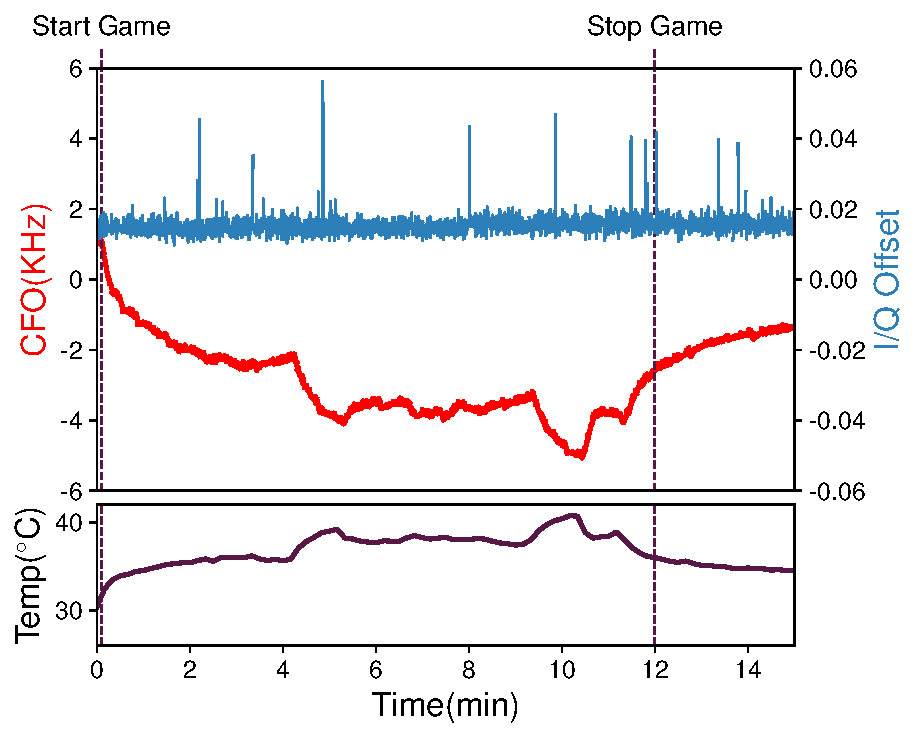
\includegraphics[width = \textwidth]{bletracking/plots/gameplay_temp_cfoiq.pdf} 
    \caption{}
    %\caption{Metric stability while playing a GPU-intensive game}
    %\label{fig:exert_cfo}
\end{subfigure}
\hfill
\begin{subfigure}{0.48\textwidth}
    %\centering
    %\captionsetup{justification=centering}
    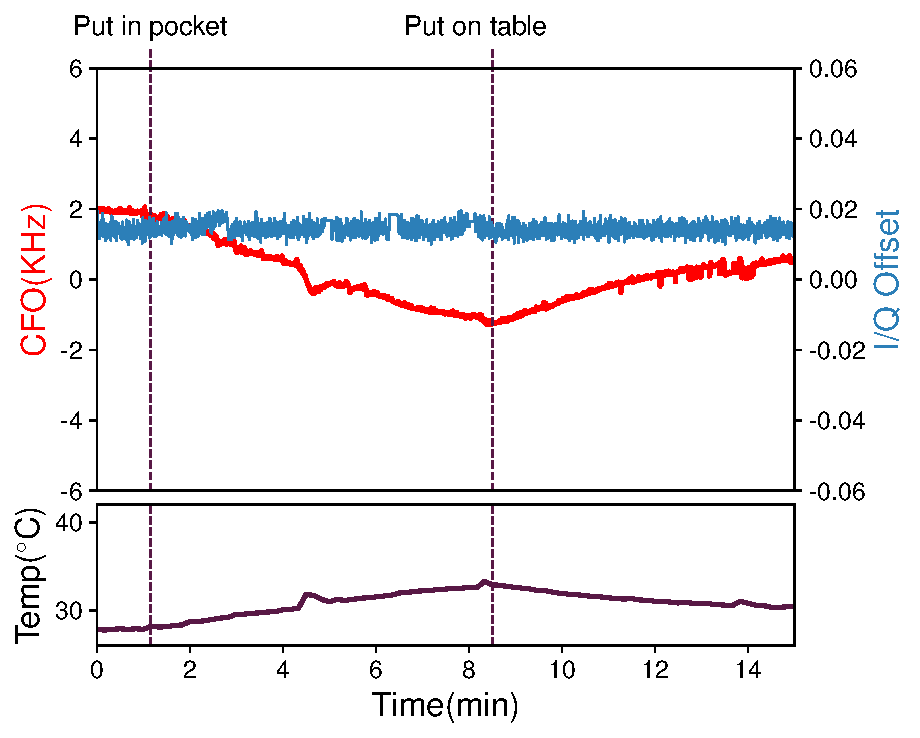
\includegraphics[width = \textwidth]{bletracking/plots/idle_temp_cfoiq.pdf} 
    \caption{}
    %\caption{Metric stability while putting the phone in a pocket}
    %\label{fig:idle_cfo}
\end{subfigure}
\captionsetup{justification=centering}
\caption{Stability of CFO and \iq offset when (a) playing a GPU-intensive game and (b) putting the phone in a pocket}
\label{fig:stability_cfo_temp}
\end{figure}

Figure~\ref{fig:stability_cfo_temp} shows the per-packet
variation in CFO and IQ offset during the 15-minute tests. We do not show the
variation in I/Q imbalance as it as we found it has a similar relationship to
temperature as I/Q offset. 
%
For the game experiment, we observe that the CFO
has a linear relationship to the changes in
temperature. When the game begins, the CFO increases, and when the game ends, it decreases.
At the peak internal temperature (+10\textdegree C above baseline),
we observe a significant CFO deviation (7~kHz).
%
%Finally, when the user stops playing the game, the temperature as well as CFO
%slowly taper off towards their initial values.
%
For the in-pocket experiment, the peak change in CFO is much
less than the game experiment (2~kHz). However, it is
still significant enough to introduce confusion with other devices that have
similar I/Q metrics (Figure~\ref{fig:cfoiq}).
Finally, figure~\ref{fig:stability_cfo_temp} show that I/Q offset
(and I/Q imbalance which is not shown) does not correlate with
temperature in both the cases.

\subsubsection*{Summary} 
Device temperature changes significantly change the CFO
a smartphone, but not the \iq imperfections. If an attacker tries to track a device when it is under
heavy use, it will need to allow for significant differences in CFO from the
initial fingerprint, which may result in increased confusion with other nearby
devices. Also, putting an idle device in a user's pocket changes the CFO
significantly enough to cause confusion as well.  Ideally, an attacker would
both get an initial fingerprint, and try to identify the device, in the of the most common use case for the device: idle in
the user's pocket. 
%If a device experiences a significant change in ambient temperature, the
%attacker would have to acquire a new fingerprint, and if the device is active, when its identified.

%}}}

\subsection{Differences in BLE transmitter power} %{{{

BLE transmit power affects how far away an attacker can track a target.  If
some devices have lower transmit power, it is more difficult for an
attacker to capture their beacons.  One may assume that all similar devices
(e.g., smartphones) would use similar transmit power---especially when they are running the same popular
app. In particular, we would expect similar transmit power for
the same contact tracing apps, where transmit power correlates with distance where the
contact occurred.  However, transmit power is configurable: BLE
APIs on mobile devices allow applications to set their beacon transmit power
to match the needs of the application.

We measured the received SNR of BLE beacons from several popular smartphones while they were
running the Apple/Google COVID--19 contact tracing app.  The measurement was
performed with a USRP N210, and all the phones were placed at the same distance (15 feet) from the
USRP. We performed this measurement on five different phones, running latest
version of iOS and different versions of Android. We installed the same
official California COVID--19 contact tracing app on all the devices. Then,
we averaged the SNR over 100 received packets
from each of the devices.

Figure~\ref{fig:txpwr} shows that the iPhone~8 has an SNR 10~dB higher
than all other Android phones we tested. Therefore, the iPhone's BLE beacons
are likely to be received considerably farther away than the other devices.
Anecdotally, we observed that an iPhone's COVID--19 contact tracing beacons
7~meters farther than any of the Android devices we tested\footnote{Including other versions of the iPhone available at the time (e.g., Xr).}.

\subsubsection*{Summary} There can be significant differences in BLE transmit power
across devices, and even across apps running on devices. We observed
that iPhones transmit COVID--19 contact tracing beacons with significantly higher
power than Android devices.  Consequently, attackers may be able to track
iPhones from a farther distance than Android devices.
%}}}

\subsection{Quality of an attacker's sniffer radio} %{{{
    \label{sec:hadi:sdr}

\begin{figure}
    \centering
    \captionsetup{justification=centering}
    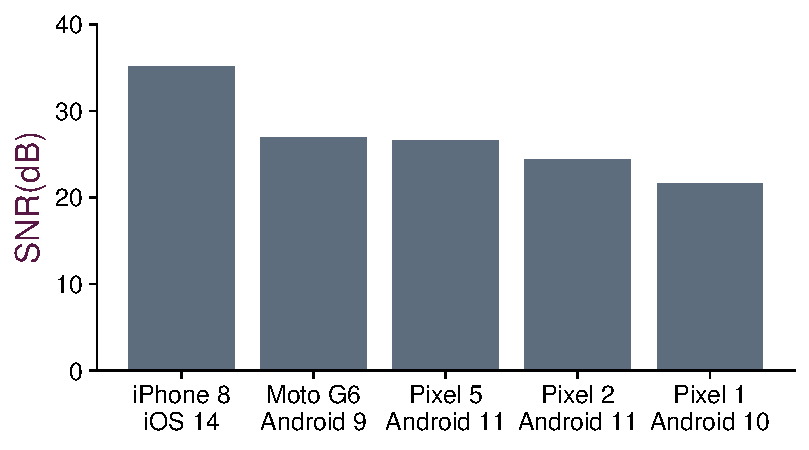
\includegraphics[width=0.6\textwidth]{bletracking/plots/phone_power_barplot}
    \caption{SNR of COVID contact tracing beacons across devices}
    \label{fig:txpwr}
    \end{figure}
    
\begin{comment}
Physical-layer fingerprinting attacks can require an expensive high-quality Software-Defined Radio (SDR) to execute.
%
The more expensive the required SDR is, the fewer locations an attacker can deploy them to track their target.
%
On the other hand, the problem is that an SDR's receiver
chain adds signal imperfections to the received signals.


Recently, several low-cost SDRs have
become popular among hobbyists.
%
However, the stability of their receivers'
imperfections are unknown. We evaluate if one of the least expensive SDRs has
sufficient imperfection stability for BLE device tracking.
\end{comment}

Physical-layer fingerprinting attacks can require an expensive high-quality
Software-Defined Radio (SDR) to execute. The problem is, an SDR's receiver
chain adds signal imperfections to the transmitted signals. If the SDR's
imperfections are unstable, they can make it difficult to identify a device
based on its previously captured fingerprint. On the other hand, the more expensive the required SDR is, the fewer locations an attacker can
deploy them to track their target. 

Recently, several low-cost SDRs have
become popular among hobbyists. However, the stability of their receivers'
imperfections are unknown. We evaluate if one of the least expensive SDRs has
sufficient imperfection stability for BLE device tracking.

We compared the fingerprinting metrics captured by a high-end SDR, USRP N210 (\$3,400), and a low-end SDR, LimeSDR-Mini (\$179).
To make the comparison fair, we sent BLE packets from a single iPhone device to both SDRs simultaneously.
We computed the average and standard deviation of
our metrics to evaluate if the two devices observe the same absolute imperfections, and if they have similar metric stability.
Similar to prior experiments, we captured 100 beacons to compute these
distributions.

\subsubsection*{CFO} The USRP observed a mean of -4.78~kHz and a standard
deviation of 102~Hz, while the Lime-SDR observed a lower mean of -8.07~kHz
but with a similar standard deviation of 114 Hz. The difference is in the mean CFO is likely due
to manufacturing variations in the SDR's crystal oscillators. Both radios
however use a TCXO-based oscillator, therefore their CFO measurements will be stable even if the SDR's temperature changes.

\subsubsection*{\iq metrics} A similar conclusion can be drawn about the
differences between the observed I/Q metrics. The USRP observed an average I/Q
offset magnitude of 0.0145 and standard deviation of 0.0017. While the Lime-SDR
observed an average of 0.0203 but with a similar standard deviation 0.0030. 
The \iq imbalance was surprisingly similar across both devices, with a mean
amplitude of 0.991 for the USRP and 0.987 for the Lime-SDR, the corresponding standard deviations
were similar too (0.0016 and 0.0021).

\subsubsection*{Summary} Attackers can use lower-cost (\$179) hobbyist-grade
SDRs to do physical-layer attacks, but they will likely have to calibrate the
differences between their SDRs before they deploy them.
%}}}

\subsection{Mobility of target device} %{{{
\label{sec:hadi:mobility}

Physical-layer tracking would be impossible if the BLE fingerprint of BLE device
changes as it moves from one physical location to another.  Specifically,
fingerprints may change due to differences in the target's physical environment
(e.g., multipath in one room vs. another), and differences in
motion of the target (e.g., walking vs. driving).
    
\subsubsection*{Physical environment} A change in the physical location of the
target can alter the received signal's SNR due to changes
multipath conditions. However, we observed that this appears to have 
an insignificant impact on BLE fingerprinting metrics. 
%
We have observed through experiments that above a
certain minimum SNR ($\sim$10 dB), changes in SNR do not impact
identification accuracy.

\subsubsection*{Speed of Motion} A moving BLE device may experience a
velocity-dependent frequency offset due to the Doppler
effect~\cite{nasadoppler}. While this may cause a slight drift in the CFO of
the BLE target device, the impact is not significant for the frequencies that
BLE operates at. 

For example, if a BLE device is moving at a velocity of 80
kilometers per hour,  and the receiver is stationary, the Doppler frequency
offset at 2.4~GHz is about 180 Hz. This is only \~50\% of the median of standard
deviation of CFO for BLE devices we observed in the field
(Figure~\ref{fig:cfo_comp}). Therefore, even at
relatively high speed motion, the Doppler shift doesn't impact an attacker's
ability to track devices.
    
\subsubsection*{Summary} 
Changing location, or speed, of BLE device has an insignificant impact on the
attacker's ability to accurately fingerprint and identify a target device.
    
    %\begin{figure}[t!]
        %\centering
        %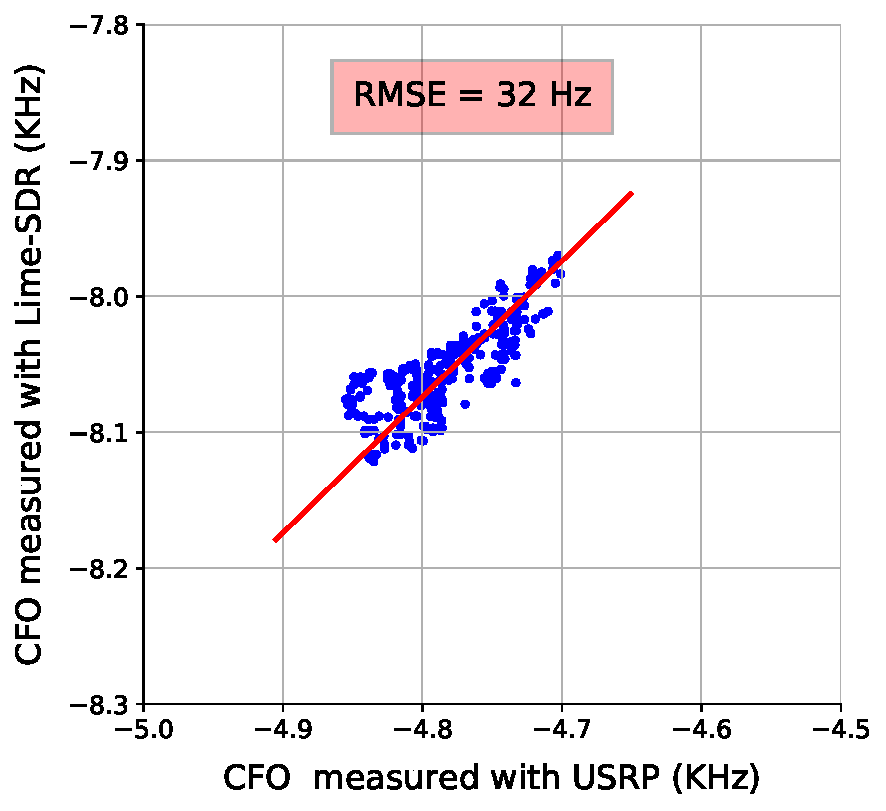
\includegraphics[width = \linewidth]{plots/cfo_scatter_sdr.pdf}
        %\caption{CFO Comparison of two SDR receivers. CFO values of 1000 packets from a device were measured with a Lime-SDR and an USRP. The RMSE is 32 Hz which indicates it is possible to use a different receiver as long as the CFO between receivers is calibrated compensated.}
        %\label{fig:cfo_scatter_sdr}
    %\end{figure}
%}}}
    
